\section{Prototypage}
\subsection{Implémentation}
\begin{frame}
 \frametitle{Prototypage}
 Un réseau de capteurs sans fil a été déployé dans une maison pendant 12 jours dans un contexte de gestion d'énergie.
 L'implémentation de leur prototype ne requiert que 15,8k, parseur XML, serveur HTTP et file TCP/IP inclus !
 \begin{figure}
  \centering
  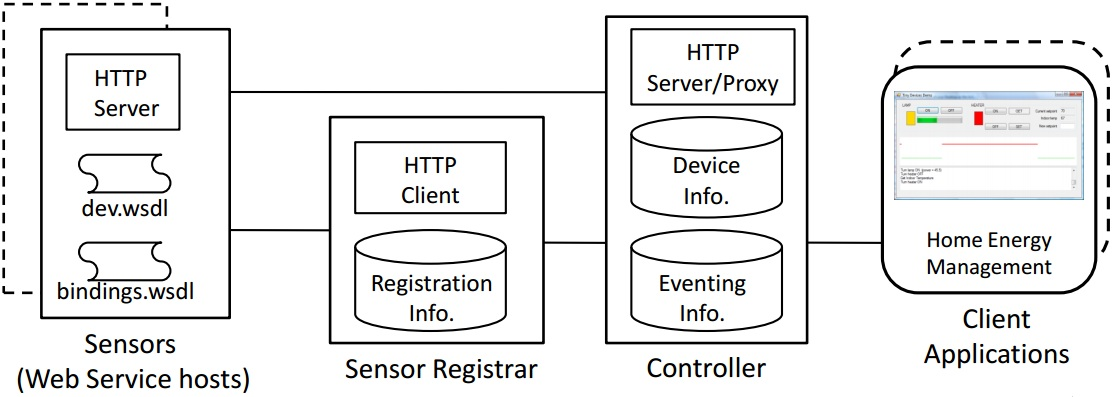
\includegraphics[scale=0.36]{figures/implementation.jpg}
  \caption{Diagramme d'implémentation du service web}
 \end{figure} 
\end{frame}

\newcommand{\unite}{(octets)}
\begin{frame}%[fragile]
 \frametitle{Implémentation}
 \framesubtitle{Mémoire utilisée}
 \begin{center}
 \begin{tabular}{|l|r|r|r|}
  \hline
  Module & Code & Data & Const\\
  ~ & \unite & \unite & \unite \\
  \hline
  Librairies & 804 & 2 & 76\\
  controle hardware & 408 & 78 & 12\\
  Driver radio & 4282 & 404 & 14\\
  TCP/IP & 2964 & 332 & 4\\
  Serveur web+parseur XML & 2380 & 54 & 4864\\
  \hline
  \textbf{Total} & \textbf{10838} & \textbf{870} & \textbf{4970}\\
  \hline
 \end{tabular}
 \end{center}
\end{frame}

%TODO description de figure 11

\subsection{Déploiement}
\begin{frame}
 \frametitle{Déploiement}
 Le réseau de capteurs déployé contient aussi des capteurs communément utilisés pour la sécurité.
 Par exemple, ils ont utilisés des capteurs de mouvement, d'ouverture de porte, ...
 Mais ils ont également placé des capteurs permettant de mesurer et regler la consomation d'énergie de n'importe quel appareil grâce à leurs \textit{smart-sockets}.
\end{frame}

\newcommand{\smartsocket}{\textit{smart-socket}~}
\begin{frame}
 \frametitle{Diagramme du \smartsocket}
 \begin{figure}
  \centering
  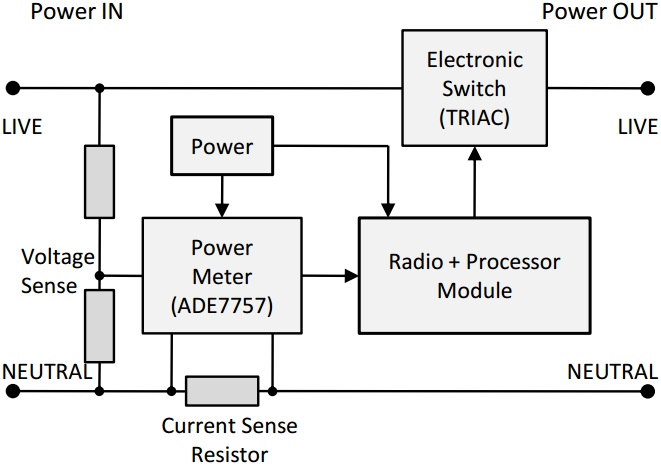
\includegraphics[scale=0.35]{figures/smartsocket.jpg}
  \caption{Le \smartsocket}
 \end{figure} 
 À brancher au réseau électrique, le \smartsocket permet de mesurer l'énergie électrique consommée par l'appareil branché au \smartsocket et de l'éteindre ou l'allumer à distance.
 Il supporte jusqu'à 2kW\\
 %On a besoin de visualiser la consomation d'énergie de chaque appareil.
 %Combiné avec des capteurs d'ouverture de porte et capteur de mouvements, un algorithme de gestion d'énergie peut être appliqué.
 %Lors de l'expérience, des smart-sockets ont été utilisés pour les lampes et appareils de divertissement utilisés la plupart du temps.
\end{frame}

\def \exsca {0.21}
\begin{frame}
 \frametitle{Quelques données collectées\footnote{L'unité de l'axe du temps n'est pas affiché pour protéger la vie privée des résidents.}}
 \begin{figure}
  \begin{minipage}[c]{.46\linewidth}
   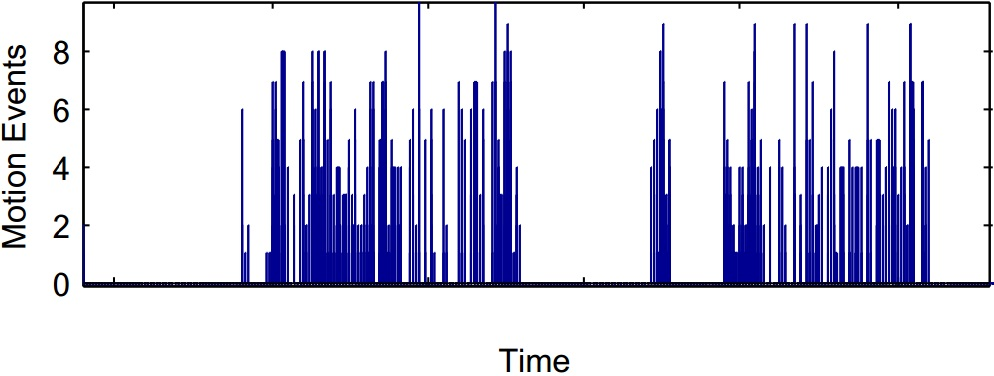
\includegraphics[scale=\exsca]{figures/EXmovement.jpg}
   \caption{Détecteur de mouvements}
  \end{minipage}
  \begin{minipage}[c]{.46\linewidth}
   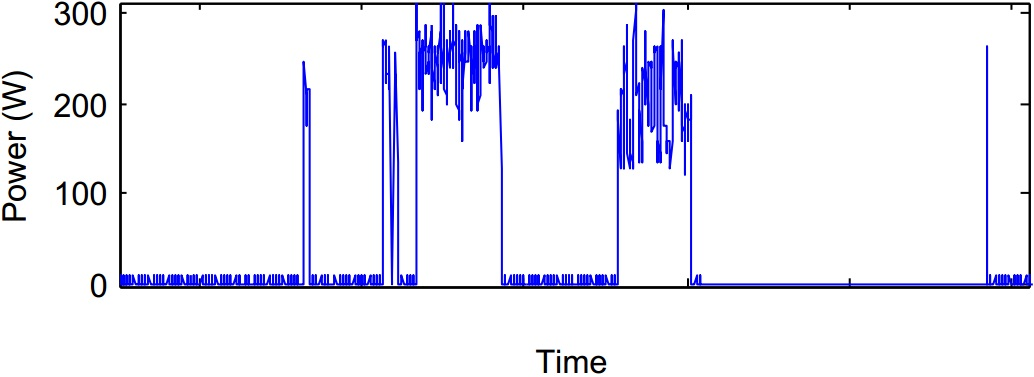
\includegraphics[scale=\exsca]{figures/EXpower.jpg}
   \caption{\smartsocket de la lampe}
  \end{minipage}
 \end{figure}
 \begin{figure}
  \centering
  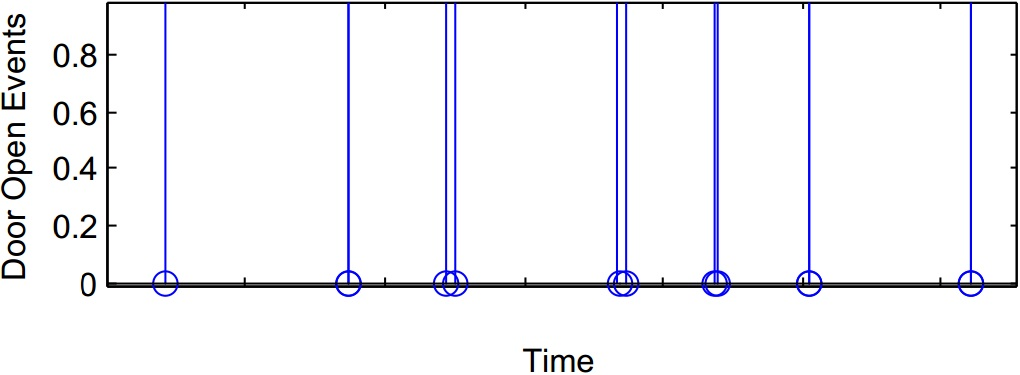
\includegraphics[scale=\exsca]{figures/EXdoor.jpg}
  \caption{Ouverture de la porte}
 \end{figure}
\end{frame}

\begin{frame}
 \frametitle{Résultats}
 Grâce à un algorithme qui baisse la température du chauffage lorsque la maison est innocupée, ils ont pu économiser 7,2\% d'énergie de chauffage.
 Le graphique suivant montre l'économie totale d'énergie par jour.
 \begin{figure}
  \centering
  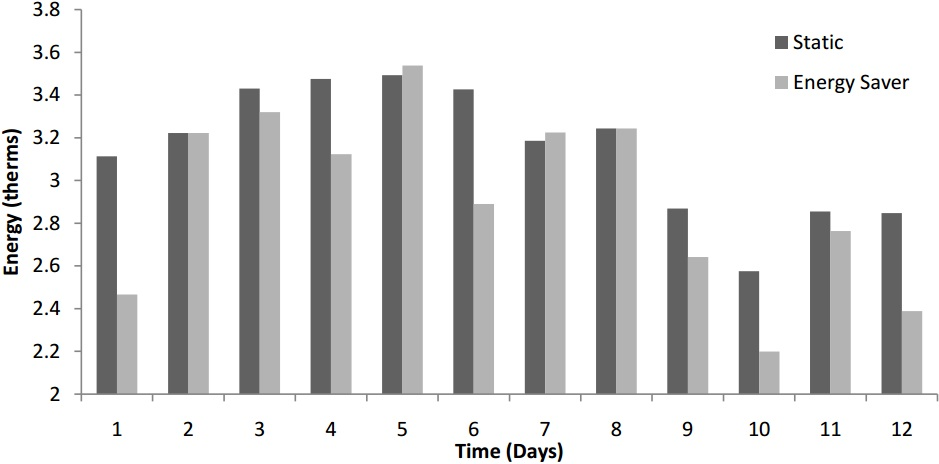
\includegraphics[scale=0.38]{figures/energysaver.jpg}
  \caption{Économie d'énergie totale}
 \end{figure} 
 Ils ont utilisé un algorithme se basant que sur l'occupation de la maison. Il existe de meilleurs algorithmes prenant en compte l'occupation de chaque pièces.
\end{frame}

 
 